% !TEX root = ../my-thesis.tex
%
\chapter{Definizione del problema e lavori correlati}
\label{sec:literature_review}

Lo scopo del lavoro di questa tesi è quello di costruire un sistema software che analizzi testi documentali scritti in linguaggio naturale con l'obbiettivo di estrarre dati in formato RDF (triple) che possano essere aggiunti ai dati di una base di conoscenza.

Questo progetto rientra nell'ambito della \textit{Knowledge Base Construction}.
Il processo di costruzione di una base di conoscenza si compone di due operazioni fondamentali: l'architettura e il popolamento. 

In particolare ci si è concentrati sulla risoluzione del problema del popolamento, denominato convenzionalmente come \textit{KBP (Knowledge Base Population)}, prendendo in oggetto basi di conoscenza già costruite seguendo il modello Linked Data.

Il tema KBP è attualmente oggetto di ricerca come dimostrato dall'impegno del NIST (National Institute of Standards and Technology) nel riproporre, nel convegno annuale TAC\cite{TAC}, un workshop rivolto ad alimentare la ricerca in questo settore. In particolare è di interesse, per il progetto di questa tesi, il task \textit{Slot Filling}, che prevede il popolamento di una base di conoscenza a partire da \textit{entità} e \textit{proprietà} note (Sezione \ref{sec:intro:web_history}).

Il popolamento di basi di dati Linked Data costituisce una specializzazione del problema KBP. I progetti maggiormente impegnati in quest'ambito sono YAGO\cite{Suchanek2007YagoAC} e DBpedia\cite{Lehmann2015DBpediaA}. Quest'ultimo ha contribuito ad incentivare la ricerca in quest'area tematica proponendo nell'anno 2017 la competizione \textit{TextExt - DBpedia Open Extraction Challenge}\cite{DBpedia_TextExt}.

KBP fa parte dell'ambito di ricerca più generico denominato \textit{IE} (Information Extraction), che riguarda l'estrazione di informazioni strutturate da testi in linguaggio naturale.

Nel seguito di questo capitolo vengono descritti i lavori e le tecniche presenti in letteratura che hanno motivato questo progetto.


%Quello della costruzione di basi di conoscenza è un ambito dell'Intelligenza Artificiale studiato già da prima della formulazione del concetto di Web. L'interesse per questo strumento è nato dall'esigenza di strutturare i dati in maniera ben organizzata, facilmente consultabile da tutti e processabile dai computer. La nascita del Semantic Web ha reso possibile per le basi di conoscenza di essere distribuite, collegate e uniformemente strutturate.

%Il requisito delle basi di conoscenza di essere agevolmente consultabili da tutti marca una netta differenza con i database, in cui i dati e le loro relazioni sono noti ai soli tecnici e sono architettati al fine della progettazione del software.
%I documenti testuali, pur raccogliendo conoscenza fruibile a tutti, non soddisfano invece il requisito \textit{machine readable}.
%I database e i contenuti testuali documentali rappresentano la sorgente dati delle basi di conoscenza.

%Un esempio di costruzione di basi di conoscenza a partire da basi di dati è stato già descritto nella sezione \ref{sec:intro:linked_data_production}, mostrando che è un compito già automatizzabile, diffuso (nelle organizzazioni governative) e privo di problemi rilevanti.













\section{Information Extraction}
\label{sec:literature_review:information_extraction}

L'Information Extraction si occupa di identificare le entità presenti in un testo e i fatti asseriti che le riguardano al fine di estrarre informazioni strutturate. Le tecniche utilizzate rientrano nell'ambito di quello che viene chiamato \textit{Natural Language Processing} (\textit{NLP}).

L'estrazione di dati strutturati da testo libero si compone di due sottoproblemi: la scoperta delle menzioni delle \textit{entità} di interesse (\textit{entity mentions}) e l'identificazione delle \textit{relazioni} che le riguardano (\textit{relation mentions})\cite{Grishman2012InformationEC}.

Le menzioni da ricercare sono di tre tipi:
\begin{itemize}
\item \textit{Named Mentions}: menzioni dei nomi delle entità ricercate (es. "Francesco Totti"). 
\item \textit{Pronoun Mentions}: menzioni ad entità tramite pronomi.
\item\textit{Nominal Mentions}: menzioni ad entità di tipo nominale (es. "l'ottavo re di Roma").
\end{itemize}
Le tecniche rivolte al riconoscimento e classificazione del primo tipo di menzioni vengono definite \textit{Named Entities Recognition} (\textit{NER}), mentre per gli altri due tipi si parla di \textit{Coreference Resolution}.

Nell'ambito della NER vengono convenzionalmente definite delle categorie standard. Le più comuni sono \textit{PERSON} per le persone, \textit{GPE} per le entità geografiche e politiche, \textit{ORGANIZATION} per le organizzazioni. Anche le espressioni temporali vengono considerate come categoria della NER (\textit{DATE}). 
Fare NER significa individuare nel testo le named entity e dedurne la categoria di appartenenza.
Ad oggi la tecnica NER è implementata nella maggior parte dei software di NLP ed ha raggiunto risultati accurati sia a livello di precisione che di richiamo.
 

Quello della coreference resolution è un problema ancora aperto, specialmente per le lingue diverse da quella inglese. Questo tipo di tecnica prevede il riconoscimento di riferimenti ad entità che non sono espliciti, ma avvengono tramite quelle che in linguistica vengono definite \textit{anafore}. Tale problema è molto condizionato dalle specificità delle lingue, dal tipo di contesto ed è difficile da valutare. Per queste ragioni non molti software NLP implementano questa funzionalità e se lo fanno è generalmente disponibile in poche lingue ed ha scarsa efficacia.

Il problema dell'identificazione delle menzioni di relazioni riguarda invece la ricerca di predicati o proprietà che associano le entità tra loro. Per le coppie di entità di tipo PERSON, una relazione potrebbe essere quella di essere sposati. Questa relazione può essere espressa in vari modi ed etichettata con annotazioni di diversa provenienza che tuttavia hanno lo stesso valore semantico. Il legame coniugale, ad esempio, può essere rappresentato dall'arbitraria annotazione "essere\_sposati" o da un \textit{frame semantico} o da una proprietà o predicato definito in una tassonomia come la proprietà \textit{dbo:spouse} presente nell'OWL di DBpedia.

Le tecniche che cercano di risolvere questo problema a livello linguistico/semantico rientrano nell'ambito del \textit{semantic role labeling}.
Solitamente queste tecniche sono di apprendimento automatico supervisionato allenato su corpus testuali manualmente annotati con frame semantici come \textit{FrameNet} \cite{FrameNet} o \textit{PropBank}\cite{Kingsbury2002FromTT}.
Nella KBP di Linked Data la relation extraction è di fondamentale importanza. Le relazioni da scoprire sono definite nelle ontologie sotto forma di predicati: la procedura consiste nel collegare (\textit{linking}) caratteristiche di una proposizione testuale (features linguistiche) ad un predicato già definito.

La risoluzione dei problemi precedentemente descritti non può prescindere da una preventiva analisi del testo tramite NLP. Tale analisi prevede vari passaggi sequenziali che estraggono \textit{features} linguistiche utilizzate come input per il passo successivo. Si inizia suddividendo il testo in frasi e si prosegue suddividendo le frasi in \textit{token}. La generazione di token (\textit{tokenization}) ha il compito di tagliare una sequenza di caratteri in segmenti significativi, escludendo alcuni tipi di caratteri non desiderati come i simboli di punteggiatura. Successivamente avviene l'analisi dei \textit{chunk}: blocchi di token che rappresentano parti sintattiche del discorso (\textit{Part of speech}). I vari chunck vengono analizzati con delle regole grammaticali per costruire un albero delle dipendenza sintattiche.

Le features linguistiche prodotte dal processo NLP vengono sfruttate nell'IE per implementare la scoperta e la classificazione delle entità e successivamente, per ogni coppia di entità, per dedurre la relazione corretta. L'intero processo appena descritto è rappresentato nella figura \ref{fig:literature_review:ie} 
%Controllare numero aggiungere vertical space e riquadro

\begin{figure}[htb]
\fbox{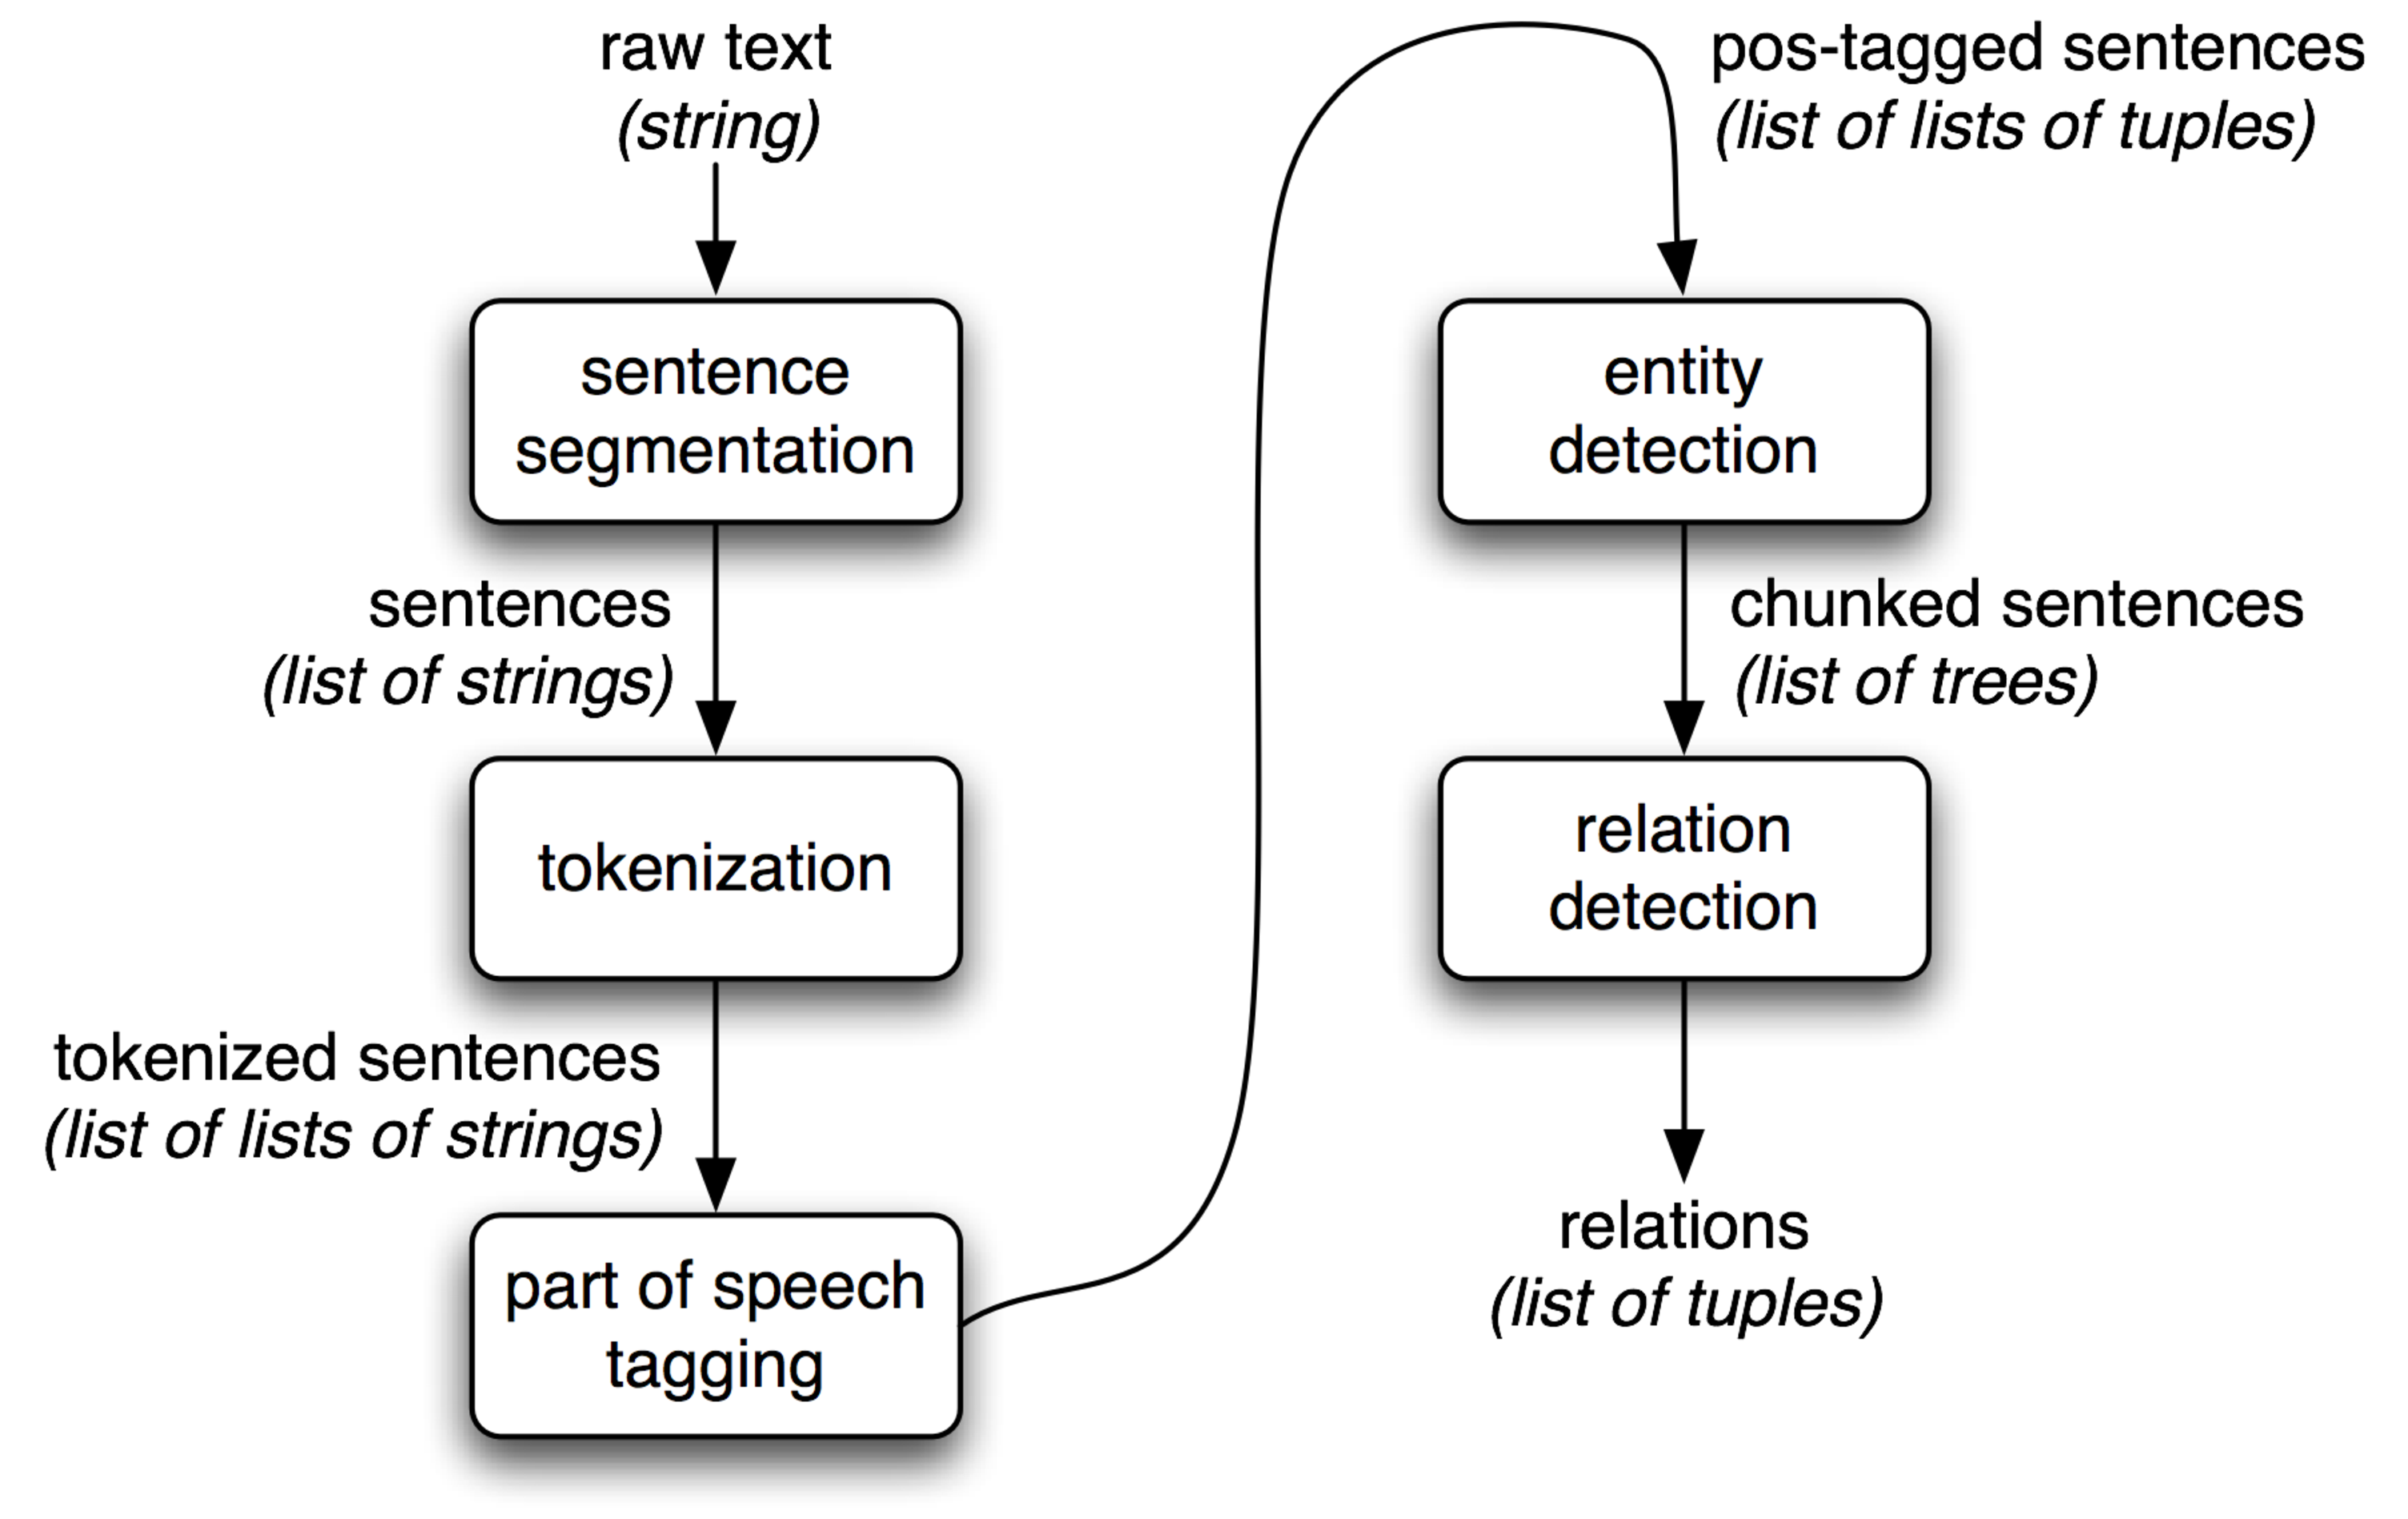
\includegraphics[width=\textwidth]{gfx/ie-architecture.pdf}  }
	\caption{Processo di Information Extraction}
\label{fig:literature_review:ie}
\end{figure}

Le strategie che sfruttano features linguistiche nell'ambito dell'IE sono:
\begin{itemize}
\item Regole programmate a mano.
\item Apprendimento supervisionato in cui tutti i dati di training sono etichettati.
\item Apprendimento non supervisionato in cui non si fa uso di insiemi di training.
\item Apprendimento semi-supervisionato in cui solo una parte dell'insieme di training è etichettato.
\end{itemize}
Le regole programmate a mano, come noto, pur essendo efficienti in casi particolari, si dimostrano inattuabili se il problema da modellare ha un input troppo esteso o dipende da un elevato numero di fattori.

Se da un lato l'apprendimento supervisionato mostra ottimi risultati, dall'altro si rivela attuabile solo se esistono insiemi di training naturalmente etichettati. E' il caso, per esempio, del semantic role labeling usando corpus annotati con semantic frame. L'operazione di etichettare i dati a mano può essere molto dispendiosa in casi come quello della KBP in cui le classificazioni da fare (i diversi tipi di relazioni da scoprire) sono numerose.

I sistemi di apprendimento non supervisionato si basano solamente sulle caratteristiche dell'input e non su dati precedentemente etichettati. Nell'ambito dell'IE non vengono utilizzate frequentemente a causa della scarsa efficienza e della difficoltà nella valutazione dei modelli prodotti. 

In alternativa si usano procedure semi-supervisionate in cui si prende in input un piccolo insieme etichettato (L) ed un altro non etichettato (U). Generalmente l'apprendimento semi-supervisionato si basa sull'avere un classificatore che non solo può classificare nuovi dati, ma può stimare il livello di fiducia nella sua classificazione. Il processo funziona in modo iterativo, aumentando gradualmente l'insieme L e quindi migliorando il classificatore. Ad ogni iterazione, il classificatore viene allenato su L, applicato ad U, generando nuove etichette la cui affidabilità viene valutata. Le nuove etichette con livello di confidenza più alto vengono aggiunte ad L, mentre le altre restano in U. Un limite di questo sistema è il riconoscimento di un'adeguata condizione di terminazione. Per favorire una corretta valutazione delle etichette prodotte viene talvolta sfruttata la tecnica di \textit{Active Learning}, in cui le etichette vengono valutate interattivamente da un agente umano.

Un tipo di apprendimento semi-supervisionato molto particolare e utilizzato in ambito IE è la \textit{Distant Supervision}. Questa tecnica consiste nel costruire un insieme di training interrogando automaticamente una base di conoscenza. Una volta costruito l'insieme di training, si effettua un allenamento e una classificazione in maniera supervisionata. Tecniche di questo tipo, che permettono la classificazione non disponendo di una base di verità (\textit{ground truth}), bensì cercando di approssimarla, rientrano nella categoria definita come \textit{weak supervision}.
Tali tecniche sono soggette alla produzione di etichette con presenza di rumore o con una bassa copertura. A tal proposito, un problema attualmente aperto, è quello di cercare di coniugare i segnali prodotti dall'azione di varie tecniche di questo tipo in un unico risultato \cite{Ratner2017SnorkelFT}.

Citando \citet{Grishman2012InformationEC}, bisogna tenere in mente che, anche se in alcuni casi l'apprendimento completamente automatico batte i migliori sistemi programmati a mano, in molti casi la congiunzione di machine learning e regole esplicitamente programmate è difficile da superare. Il progetto di questa tesi si ispira a questa idea, prevedendo infatti un approccio che affianca regole programmate in maniera esplicita con strumenti di classificazione semi-supervisionata come la distant supervision.

\subsection{Distant Supervision}
\label{sec:literature_review:information_extraction:distant_supervision}
Un tipo di apprendimento semi-supervisionato che ha ricevuto molta attenzione nella letteratura riguardante IE, ed in particolare in KBP, è quello denominato \textit{\textbf{Distant Supervision}}. Questa tecnica si basa sull'assunzione di poter fare affidamento su una base di conoscenza contenente istanze della relazione d'interesse e su un corpus di testo di grandi dimensioni contenente menzioni a molte delle istanze della base di conoscenza. Usando questa combinazione si possono costruire automaticamente insiemi di istanze positive e negative per la classificazione di relazioni. 

Questo approccio è stato descritto come "learning from weakly labeled data" [CK99] e più recentemente soprannominato \textit{Distant Supervision} \cite{Mintz2009DistantSF}.
Il nome deriva dal fatto che la base di conoscenza fornisce supervisione, ma non tramite annotazione diretta dei dati di testo. 

Nell'etichettamento (\textit{labeling}) dell'insieme di allenamento si prendono le istanze [Soggetto, Oggetto] della relazione nella base di conoscenza e si raccolgono tutte le proposizioni nel corpus testuale contenenti entrambe le menzioni alle due entità. Tali segmenti di testo diventano gli esempi etichettati positivamente, le restanti proposizioni vengono etichettate come negative. L'insieme prodotto viene poi utilizzato per allenare ed applicare un classificatore allo stesso modo di un approccio supervisionato.

La distant supervision è in grado di produrre una grande quantità di dati di training che potrebbero però essere rumorosi. Questa tecnica presenta i seguenti problemi:
\begin{itemize}
\item per una coppia di entità potrebbero sussistere più tipi di relazione. Questa caratteristica deriva in una produzione di etichette di training erroneamente positive e una conseguente generazione di classificazioni \textit{false positive}.
\item La base di conoscenza può essere incompleta. In tal caso molte frasi, che dovrebbero essere etichettate come positive, vengono scartate, implicando un numero elevato di \textit{falsi negativi}.
\item Il risultato finale è influenzato dall'accuratezza dell'\textit{entity linking} tra la menzione testuale e il valore dell'entità nella base di conoscenza (Es. collegare la menzione "Plant" all'entità "Robert Plant"). Tale operazione può essere soggetta ad \textit{overfit}, scartando menzioni valide o \textit{underfit} collegando erroneamente menzioni a entità. 
\end{itemize}




\section{Knowledge Base Population}
\label{sec:literature_review:kbp}

Con il termine \textit{KBP} (\textit{Knowledge Base Population}) ci si riferisce al problema di:
\begin{enumerate}
\item estrarre dal testo libero nuove informazioni riguardanti entità della KB;
\item strutturare le informazioni estratte secondo il modello della KB;
\item aggiungere le nuove informazioni strutturate alla KB.
\end{enumerate}

L'impegno nella risoluzione del problema di KBP è stato ripetutamente alimentato e rilanciato dal \textit{NIST} (\textit{National Institute of Standards and Technology}) nella conferenza annuale \textit{TAC} (\textit{Text Analysis Conference}). TAC è composta
da una serie di seminari organizzati per incoraggiare la ricerca nell'elaborazione del linguaggio naturale (NLP) e lo sviluppo delle relative applicazioni\cite{TAC}. TAC prevede anche un insieme di competizioni note come \textit{tracks}, ognuna delle quali si concentra su un particolare sottoproblema di NLP, come la Knowledge Base Population.

Questa competizione è stata avviata anche nell'ultima conferenza del 2017 e si compone di quattro task:
\begin{enumerate}
\item \textit{Entity Discovery and Linking (EDL)}: identificare menzioni di entità (\textit{entity mentions}) e collegarle al nodo corrispondente nella base di conoscenza.
\item \textit{Slot Filling}: dato un insieme di proprietà (\textit{slots}) trovare il valore specifico per le varie entità. 
\item \textit{Event}: estrarre dal testo libero informazioni riguardanti eventi.
\item \textit{Belief and Sentiment}: individuare opinioni e sentimenti di entità nei confronti di altre entità, relazioni o eventi.
\end{enumerate}

Il lavoro di questa tesi punta a dare un contributo esclusivamente ai primi due task, con la particolarità che le entità e gli "slot" presi in considerazione sono le entità e i predicati del mondo Linked Data.

Fare KBP su basi di conoscenza Linked Data significa estrarre proposizioni dal testo in lingua naturale che siano rappresentabili come un'asserzione (s,p,o) RDF.
Più precisamente Linked Data KBP (denominata d'ora in poi come LDKBP) è il processo che prevede di:
\begin{enumerate}
\item individuare nel testo le menzioni di entità e la loro categoria (NER),
\item collegarle le named entity estratte alle corrispondenti entità RDF appartenenti alla base di conoscenza Linked Data (entity linking), 
\item identificare le relazioni che hanno come soggetto o oggetto le entità estratte (relation extraction),
\item collegare i predicati dei vocabolari OWL, usati nella KB e trattati come input, con le relazioni estratte (\textit{relation linking}), 
\item formare delle proposizioni RDF, da aggiungere alla base di conoscenza con le entità e i predicati estratti (slot filling o più nello specifico \textit{triples extraction}).
\end{enumerate}

Il processo LDKBP è composto da due input: il testo libero da analizzare e le proprietà Linked Data da ricercare.
L'input di tipo testuale non ha particolari requisiti o limitazioni ed è di conseguenza potenzialmente molto vasto.
Le entità e i predicati Linked Data hanno ormai raggiunto una larga definizione e rispecchiano quasi ogni entità o proprietà della realtà a noi conosciuta. Queste caratteristiche dimensionali dell'input comportano delle limitazioni nelle strategie adottabili per l'elaborazione. Le tecniche adottate sono quindi principalmente di apprendimento automatico o in alcuni casi impiegano delle regole esplicitamente programmate che sfruttano strutture deboli ricorrenti nel testo libero.

Due esempi di LDKBP che sfruttano strutture ricorrenti nel testo esaminato sono fornite da YAGO\cite{Suchanek2007YagoAC} e DBpedia\cite{Lehmann2015DBpediaA}. I due progetti hanno come corpus Wikipedia, i cui articoli consistono principalmente di testo libero, ma comprendono anche vari tipi di informazioni strutturate sotto forma di markup. Tali informazioni includono infobox, informazioni di categorizzazione, immagini, coordinate geografiche, collegamenti a pagine Web esterne, pagine di disambiguazione e collegamenti ad altre risorse o a risorse equivalenti in altre lingue. I framework dietro DBpedia e YAGO estraggono informazioni strutturate e le trasformano in dati di una base di conoscenza di dominio generico. Per potersi avvalere di queste informazioni sono state costruite delle apposite ontologie OWL con le quali mappare a mano i diversi tipi di strutture presenti. Un progetto analogo ai precedenti due, ma attualmente dismesso, è \textit{Freebase}.

Come già accennato in precedenza, per quanto riguarda l'utilizzo di machine learning in ambito di IE, si fa uso, in particolare nella letteratura più recente, della tecnica di distant supervision. 

Questa tecnica prevede l'utilizzo delle istanze di una base di conoscenza per etichettare automaticamente un insieme di training per un classificatore. Nella fase di labeling si prendono le istanze [Soggetto, Oggetto] della relazione nella base di conoscenza e si raccolgono tutte le proposizioni nel corpus testuale contenenti entrambe le menzioni alle due entità. Il testo estratto diventa parte dell'insieme di training per il classificatore.

Un iniziale approccio di questo tipo si è avuto con \citet{Craven1999ConstructingBK} nella costruzione di una base di conoscenza in ambito biologico di localizzazione subcellulare. In tale lavoro sono stati usati come input testuali i documenti del database bibliografico \textit{MEDLINE} e come risorsa per la distant supervision il database \textit{Yeast Protein Database}. Successivamente \citet{Mintz2009DistantSF} hanno usato Freebase come base di conoscenza (considerando le 102 proprietà più ricorrenti), mentre Wikipedia è stata utilizzata come fonte di testo. E' stato utilizzato un insieme di features linguistiche per allenare un classificatore in grado di avere alta precisione. Il modello è stato valutato a mano considerando le 100 o 1000 istanze estratte di maggior confidenza per ciascuna relazione dimostrando una misura F1 tra il 67\% e il 69\%.

Successivamente \citet{Nguyen2011EndtoEndRE} hanno utilizzato nel loro lavoro un sistema di valutazione più adeguato annotando 200 documenti con 52 relazioni e misurando un valore \textit{F1} pari al 67\%.

Recentemente il progetto di \citet{Cannaviccio2016AccurateFH} basato su distant supervision di articoli di Wikipedia con il database \textit{Freebase} si è posizionato al primo posto nella competizione TextExt di DBpedia. La particolarità di questo progetto è quella di avere un supporto multi-lingua e di discriminare le relazioni ,non in base alle generiche features linguistiche, ma in funzione delle cosidette \textit{typed phrase}: segmenti testuali che identificano le proprietà della base di conoscenza da popolare. Purtroppo non si conoscono dettagli sulle prestazioni di questo progetto.

\subsection{Data Programming in Snorkel}
\label{sec:literature_review:data_programming}

La distant supervision è una tecnica che permette un approccio di machine learning debolmente supervisionato creando insiemi di training quando non sono naturalmente disponibili, ma è soggetta a problemi di: incompletezza della base di conoscenza, difficoltà nell'entity linking, relazioni multiple per le entità. Tali problemi introducono rumore e bassa copertura dei dati etichettati che si riflette sulla classificazione finale.
Il paradigma \textit{data programming} \cite{Ratner2016DataPC, Ehrenberg2016DataPW,Bach2017LearningTS} è stato ideato per costruire automaticamente insiemi di allenamento, limitando la presenza di rumore e senza avere accesso ad una base di verità.
 
La tecnica di data programming è stata teorizzata, implementata e rilasciata pubblicamente dalla \textit{Stanford University} nei progetti \textit{DeepDive}\cite{Niu2012DeepDiveWK} e nella sua evoluzione \textit{Snorke}l\cite{Ratner2017SnorkelFT}. Lo sviluppo del primo progetto è stato dismesso in favore del secondo, per tale ragione ci si riferirà nel seguito della tesi al progetto Snorkel.

Snorkel viene presentato come il primo sistema "end-to-end" in grado di addestrare modelli di machine learning allo stato dell'arte senza disporre di dati etichettati manualmente. Il testo libero viene etichettato automaticamente da quelle che vengono chiamate \textit{labeling functions}: funzioni programmate, che esprimono euristiche arbitrarie e che possono avere precisione e correlazione sconosciuta. 
La tecnica di data programming permette di raffinare i segnali prodotti dalle varie labeling functions in base a quanto esse sono concordanti o discordanti, producendo un insieme etichettato con bassa presenza di rumore.

Le varie labeling function sono fonti di weak supervision e sono dei seguenti tipi:
\begin{itemize}
\item \textit{Distant Supervision}.
\item \textit{Pattern-based}: euristiche basate su un modello fornito da un esperto del dominio. 
\item \textit{Weak classifier}: classificatori insufficienti per l'intero problema, con una copertura limitata, rumore o allenati su dataset differenti.
\item \textit{Crowdsourcing}: etichette generate a mano da utenti non esperti e imprecisi.
\end{itemize}

Nella loro forma più generale, le labeling function sono semplicemente snippet di codice scritti in Python che accettano in input un oggetto \textit{Candidato} e restituiscono in output un'etichetta positiva o negativa o si astengono. Un oggetto candidato è un segmento di testo delimitato da due token (\textit{Span}) filtrato dal resto del corpus in base a delle features arbitrarie fondamentali che lo rendono plausibilmente adatto ad essere considerato come esempio da etichettare. Si consideri come esempio la relazione "essere sposato" per cui sono candidati solamente i segmenti di testo delimitati da due named entities del tipo PERSON. 

Nell'approccio di data programming, le varie funzioni di labeling descrivono implicitamente un modello generativo. Avendo dati \textit{x}, con etichette da prevedere \textit{y}, in un approccio discriminativo si modella direttamente \textit{P (y | x)}, mentre in un approccio generativo si modella \textit{P (x, y) = P (x | y) P (y)}. Nel caso specifico si modella un processo di formazione delle etichette dell'insieme \textit{P (L, y)}, dove \textit{L} sono le etichette generate dalle labeling functions per gli oggetti \textit{x}. Costruendo un modello generativo e stimando direttamente \textit{P (L | y)}, si apprende essenzialmente l'accuratezza relativa delle funzioni di labeling in base a come si sovrappongono o sono in conflitto. 

L'output di Snorkel è un insieme di \textit{probabilistic labels}, ovvero etichette con una probabilità marginale di attendibilità, che possono essere usate per allenare una larga varietà di modelli discriminativi di machine learning, come ad esempio i popolari modelli di deep learning.
Mentre il modello generativo è essenzialmente una combinazione ripesata delle labeling function fornite dall'utente, che tendono ad essere precise ma con una bassa copertura, i modelli discriminativi moderni possono conservare questa precisione incrementandone la copertura. 

Snorkel comprende funzionalità "built-in" o integrate che rendono applicabile l'intero processo di classificazione a partire dal solo corpus testuale non etichettato. Le fasi fondamentali del processo sono:
\begin{enumerate}
\item Parsing del corpus testuale con tool di NLP integrati e integrabili.
\item Estrazione degli oggetti candidati in base alle features NLP ricavate nella fase precedente.
\item Definizione e applicazione delle labeling function agli oggetti candidati.
\item Allenamento del modello generativo (built-in) con i segnali prodotti dalle labeling functions.
\item Classificazione degli oggetti candidati con il modello generativo, producendo etichette probabilistiche.
\item Allenamento di modelli discriminativi (integrati o integrabili) a partire dalle etichette probabilistiche.
\end{enumerate}
Per predire nuove etichette da esempi non conosciuti si applica nuovamente il parsing NLP, si verifica che si tratti di un oggetto candidato e si usa il classificatore discriminativo. Tra le librerie integrate in Snorkel troviamo \textit{Spacy} e \textit{CoreNLP} per il parsing e \textit{TensorFlow} per il machine learning. Le API fornite da Snorkel consentono un utilizzo semplificato ad alto livello di tali librerie.

La valutazione di Snorkel attribuisce due risultati principali:
\begin{enumerate}
\item Superamento dei risultati ottenuti con le singole tecniche di weak supervision. In particolare è stato valutato che la tecnica più popolare di weak supervision, la distant supervision, può essere superata del 132\%.
\item Creazione di un nuovo paradigma di interazione per la costruzione di insiemi etichettati. E' stato dimostrato empiricamente, in un workshop della durata di due giorni, come utenti possano imparare in così breve tempo a produrre labeling function che ottengono etichette con accuratezza da subito in linea o addirittura superiore a quelle prodotte manualmente in settimane o mesi di lavoro.
\end{enumerate}

I rilevamenti alla base di questi risultati sono stati effettuati nella produzione di modelli per la classificazioni in quattro ambiti diversi: 
\begin{enumerate}
\item \textit{Chem}: estrazione di relazioni tra reagenti chimici e prodotti di reazione negli abstract di PubMed.
\item \textit{EHR}: estrazione di informazioni strutturate Biomediche da referti di pazienti ospedalieri.
\item \textit{CDR}: estrazione dagli abstract di PubMed di collegamenti causali tra sostanze chimiche e malattie.
\item \textit{Spouse}: identificazione di menzioni testuali della relazione coniugale da articoli giornalistici.
\end{enumerate}

\begin{figure}[htb]
	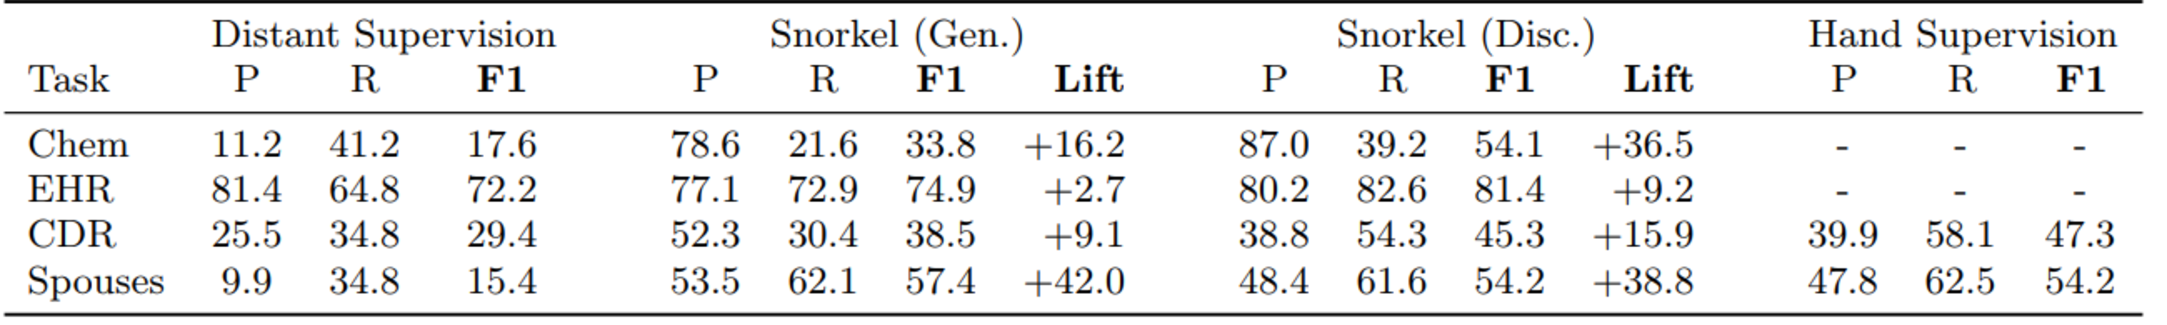
\includegraphics[width=\textwidth]{gfx/snorkel_eval.pdf}  
	\caption{\textit{Valutazione di task di estrazione di informazione dal testo.}}
	\label{fig:literature_review:snorkel_eval}
\end{figure}

I modelli generativi e discriminativi prodotti con Snorkel conseguono risultati migliori della distant supervision e mediamente equivalenti all'etichettamento a mano. Il confronto è stato misurato in termini di precisione \textit{P}, richiamo \textit{R} e media armonica delle due \textit{F1} (Fig. \ref{fig:literature_review:snorkel_eval}).

Il modello discriminativo utilizzato è di tipo \textit{Bidirectional Long Short Term Memory Network} (\textit{Bi-LSTM}) che ha dimostrato risultati allo stato dell'arte nella classificazione di input testuali in ben 22 lingue \cite{DBLP:journals/corr/PlankSG16}.

Al fine del lavoro di questa tesi è stato particolarmente indicativo il risultato raggiunto dal progetto Spouse. In tale caso le labeling functions usate sono state: distant supervision sui dati di DBpedia, modellazione di regole basate su parole chiave e pattern testuali, crowdsourcing. Questa relazione, essendo di dominio generico, è affine alle relazioni presenti in una base di conoscenza Linked Data. In funzione del risultato raggiunto da questo progetto, è lecito domandarsi se tale approccio potrebbe essere applicato al processo di LDKBP, utilizzando la distant supervision come labeling functions di default, ed ottimizzare localmente i risultati per ciascun predicato con labeling functions specifiche e con labeling functions generiche che sfruttano delle parole chiave specifiche. 










%\cite{Palomares2016WikipediaKG} \cite{Bach2017LearningTS}





%Crowdsourcing \cite{FossatiKBP}


%NLP \cite{Etzioni2004WebscaleIE}

%MINTZ The intuition ofdistant supervision is that any sentence that con-tains a pair of entities that participate in a knownFreebase relation is likely to express that relationin some way.  Since there may be many sentencescontaining a given entity pair, we can extract verylarge numbers of (potentially noisy) features thatare combined in a logistic regression classifier. Because our algorithmcan use large amounts of unlabeled data, a pair ofentities may occur multiple times in the test set.For each pair of entities, we aggregate the featuresfrom  the  many  different  sentences  in  which  thatpair appeared into a single feature vector, allowingus to provide our classifier with more information,resulting in more accurate labels. Except for the unsupervised algorithms discussedabove,  previous  supervised  or  bootstrapping  approaches to relation extraction have typically re-lied on relatively small datasets, or on only a smallnumber of distinct relations. Approaches based onWordNet have often only looked at the hypernym(is-a) or meronym (part-of) relation (Girju et al.,2003; Snow et al., 2005), while those based on theACE program (Doddington et al., 2004) have beenrestricted in their evaluation to a small number ofrelation instances and corpora of less than a mil-lion words.Hearst (1992)used a small number of regular expressions overwords and part-of-speech tags to find examples ofthe hypernym relation.  The use of these patternshas been widely replicated in successful systems,for example by Etzioni et al. (2005).The distant supervision assumption is that if twoentities participate in a relation, any sentence thatcontain those two entities might express that rela-tion.   Because  any  individual  sentence  may  givean incorrect cue, our algorithm trains a multiclasslogistic regression classifier, learning weights foreach  noisy  feature.   In  training,  the  features  foridentical  tuples  (relation,  entity1,  entity2)  fromdifferent sentences are combined, creating a richerfeature vector. In the testing step, entities are again identifiedusing  the  named  entity  tagger.   This  time,  everypair of entities appearing together in a sentence isconsidered a potential relation instance, and when-ever those entities appear together, features are ex-tracted on the sentence and added to a feature vec-tor for that entity pair.  For example, if a pair ofentities occurs in 10 sentences in the test set, andeach sentence has 3 features extracted from it, theentity pair will have 30 associated features.  Eachentity pair in each sentence in the test corpus is runthrough feature extraction, and the regression clas-sifier predicts a relation name for each entity pairbased on the features from all of the sentences inwhich it appeared. Consider  thelocation-containsrelation,  imag-ining  that  in  Freebase  we  had  two  instances  ofthis  relation:〈Virginia, Richmond〉and〈France, Nantes〉.   As we encountered sen-tences like ‘Richmond, the capital of Virginia’ and‘Henry’s Edict of Nantes helped the Protestants ofFrance’ we would extract features from these sen-tences.  Some features would be very useful, suchas the features from the Richmond sentence, andsome  would  be  less  useful,  like  those  from  theNantes  sentence.   In  testing,  if  we  came  acrossa  sentence  like  ‘Vienna,  the  capital  of  Austria’,one or more of its features would match those ofthe  Richmond  sentence,  providing  evidence  that〈Austria, Vienna〉belongs  to  thelocation-containsrelation. Our system needs negative training data for thepurposes  of  constructing  the  classifier.   Towardsthis  end,  we  build  a  feature  vector  in  the  train-ing phase for an ‘unrelated’ relation by randomlyselecting  entity  pairs  that  do  not  appear  in  anyFreebase relation and extracting features for them.While it is possible that some of these entity pairs are in fact related but are wrongly omitted fromthe Freebase data, we expect that on average thesefalse negatives will have a small effect on the per-formance of the classifier.   For performance rea-sons, we randomly sample 1% of such entity pairsfor use as negative training examples. By contrast,in the actual test data, 98.7% of the entity pairs weextract do not possess any of the top 102 relationswe consider in Freebase.We  use  a  multi-class  logistic  classifier  opti-mized  using  L-BFGS  with  Gaussian  regulariza-tion.   Our  classifier  takes  as  input  an  entity  pairand a feature vector, and returns a relation nameand a confidence score based on the probability ofthe entity pair belonging to that relation. Once allof the entity pairs discovered during testing havebeen classified, they can be ranked by confidencescore  and  used  to  generate  a  list  of  thenmostlikely new relation instances.

%Distan supervision \cite{Exner2012EntityEF} \cite{Roth2015EffectiveDS} \cite{Mintz2009DistantSF} \cite{Aprosio2013ExtendingTC} \cite{Cannaviccio2016AccurateFH} \cite{Angeli2014CombiningDA}

%TAC \cite{Surdeanu2013OverviewOT}

%TAC E DEEPDIVE \cite{Angeli2014Stanfords2S} \cite{Wu2017FonduerKB}







%The input to a KBC system is a collection of documents. The output of the system is a relational database containing facts extracted from the input and stored in an appropriate schema. To describe the KBC process, we adopt the standard terminology from the KBC community2. There are four types of objects that play integral roles in KBC systems: (1) entities, (2) relations, (3) mentions of entities, and (4) relations mentions.

%An entity e in a knowledge base corresponds to a distinct real-world person, place, or object. Entities in a knowledge base can be grouped in different entity types T1,T2,…,Tn. Entities in a knowledge base participate in relationships. A relationship between n entities is represented as an n-ary relation R(e1,e2,…,en) and is described by a schema SR(T1,T2,…,Tn) where ei∈Ti. A mention m is a span of text that refers to an entity. KBC systems typically assume that all mentions of entities in a document have a corresponding span of text that refers to them. A relation mention candidate is a particular n-ary tuple c=(m1,m2,…,mn) that represents an instance of a relation R(e1,e2,…,en) in a document. If a candidate is classified as true, it is called a relation mention, rR.













